\setAuthor{Valter Kiisk}
\setRound{piirkonnavoor}
\setYear{2006}
\setNumber{G 5}
\setDifficulty{3}
\setTopic{Gaasid}

\prob{Gaasitermomeeter}
Gaasitermomeeter koosneb mõõteampullist 1 ja manomeetrist 2, mis on omavahel ühenduses peenikese kapillaari 3 kaudu (vt joonist). Manomeetri ja mõõteampulli ruumalade suhe on $\alpha = 30$. Kapillaari ruumala võib lugeda tühiselt väikeseks. Seade täidetakse toatemperatuuril oleva gaasiga rõhuni $p_0 = \SI{1}{atm}$. Gaasi võib lugeda ideaalseks. Manomeetrit hoitakse toatemperatuuril $T_0 = \SI{293}{K}$, mõõteampull asetatakse keskkonda, mille temperatuuri on tarvis määrata. Leidke keskkonna temperatuur, kui manomeetri näit on $p = \SI{0,7}{atm}$.

\begin{center}
	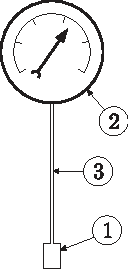
\includegraphics[width=0.25\linewidth]{2006-v2g-05-yl}
\end{center}

\hint
Kuna manomeeter ja mõõteampull on kapillaari kaudu ühenduses, siis nende gaasirõhud on isegi temperatuuride erinedes ühesugused.

\solu
Olgu mõõteampulli ruumala $V$ ning manomeetri ruumala $V_m$. Kui toatemperatuuril $T_0$ täideti seade $n$ mooli gaasiga, siis ideaalse gaasi olekuvõrrandi põhjal
\[
\frac{p_0V}{T_0} + \frac{p_0V_m}{T_0} = nR.
\]
Kuna manomeeter ja mõõteampull on kapillaari kaudu ühenduses, siis nende gaasirõhud on isegi temperatuuride erinedes ühesugused. Kui mõõteampull on temperatuuril $T$, siis (gaasi koguhulk jääb samaks)
\[
\frac{pV}{T} + \frac{pV_m}{T_0} = nR.
\]
Elimineerides $n$ ja asendades $V_m/V = \alpha$, saame
\[
T=\frac{p T_{0}}{p_{0}+\left(p_{0}-p\right) \alpha} \approx \SI{20,5}{K}.
\]
\probend